\documentclass[a4paper]{article}
\usepackage{mystyle}

\begin{document}

\customtitle{Fluctuation Strength Test Battery Experiment}

\section{Introduction}

This document describes the experimental setup proposed to obtain the data
needed regarding the tests described in the fluctuation strength test battery.
The results of pilot experiments are also reported.

\section{Results}

\subsection{AM Tones}

\subsubsection{Modulation Frequency}

Figure \ref{fig:amstds} shows the results regarding the relation between
fluctuation strength and modulation frequency by standard used. Figure
\ref{fig:amcomp} shows a comparison between the relative fluctuation strength
of the experimental data, \citeauthor{Fastl2007Psychoacoustics} data and the
proposed model.

\begin{figure}[ht]
    \centering
    \resizebox{!}{10cm}{
        % This file was created by matlab2tikz.
% Minimal pgfplots version: 1.9
%
%The latest updates can be retrieved from
%  http://www.mathworks.com/matlabcentral/fileexchange/22022-matlab2tikz
%where you can also make suggestions and rate matlab2tikz.
%
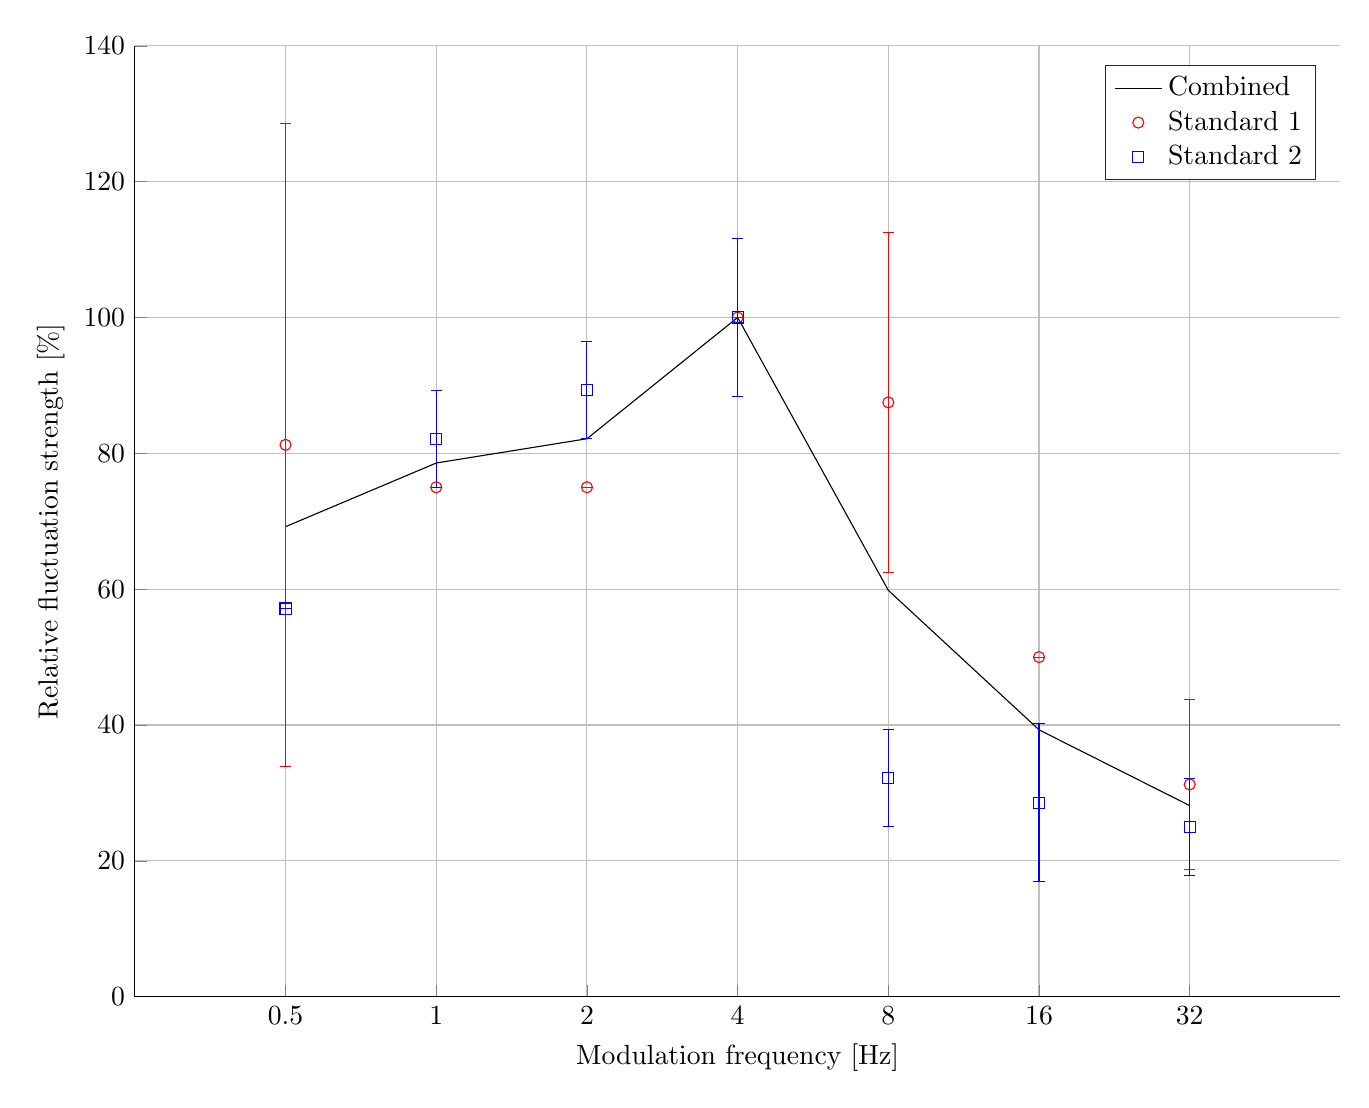
\begin{tikzpicture}

\begin{axis}[%
width=6.027778in,
height=4.754167in,
at={(1.011111in,0.641667in)},
scale only axis,
xmin=0,
xmax=8,
xtick={1,2,3,4,5,6,7},
xticklabels={{0.5},{1},{2},{4},{8},{16},{32}},
xlabel={Modulation frequency [Hz]},
xmajorgrids,
ymin=0,
ymax=140,
ylabel={Relative fluctuation strength [\%]},
ymajorgrids,
axis x line*=bottom,
axis y line*=left,
legend style={legend cell align=left,align=left,draw=white!15!black}
]
\addplot [color=black,solid]
  table[row sep=crcr]{%
1	69.1964285714286\\
2	78.5714285714286\\
3	82.1428571428571\\
4	100\\
5	59.8214285714286\\
6	39.2857142857143\\
7	28.125\\
};
\addlegendentry{Combined};

\addplot [color=red,only marks,mark=o,mark options={solid}]
 plot [error bars/.cd, y dir = both, y explicit]
 table[row sep=crcr, y error plus index=2, y error minus index=3]{%
1	81.25	47.3242362150023	47.3242362150023\\
2	75	0	0\\
3	75	0	0\\
4	100	0	0\\
5	87.5	25	25\\
6	50	0	0\\
7	31.25	12.5	12.5\\
};
\addlegendentry{Standard 1};

\addplot [color=blue,only marks,mark=square,mark options={solid}]
 plot [error bars/.cd, y dir = both, y explicit]
 table[row sep=crcr, y error plus index=2, y error minus index=3]{%
1	57.1428571428571	0	0\\
2	82.1428571428571	7.14285714285714	7.14285714285714\\
3	89.2857142857143	7.14285714285715	7.14285714285715\\
4	100	11.6642368703961	11.6642368703961\\
5	32.1428571428571	7.14285714285714	7.14285714285714\\
6	28.5714285714286	11.6642368703961	11.6642368703961\\
7	25	7.14285714285714	7.14285714285714\\
};
\addlegendentry{Standard 2};

\end{axis}
\end{tikzpicture}%
    }
    \caption{Relative fluctuation strength as a function of modulation
        frequency by standard used for AM tones with $f_c = 1$ kHz, $m_d = 40$
        dB, SPL $= 70$ dB (error bars indicate standard deviation)}
    \label{fig:amstds}
\end{figure}

\begin{figure}[ht]
    \centering
    \resizebox{!}{10cm}{
        % This file was created by matlab2tikz.
% Minimal pgfplots version: 1.9
%
%The latest updates can be retrieved from
%  http://www.mathworks.com/matlabcentral/fileexchange/22022-matlab2tikz
%where you can also make suggestions and rate matlab2tikz.
%
\definecolor{mycolor1}{rgb}{0.00000,0.44700,0.74100}%
\definecolor{mycolor2}{rgb}{0.85000,0.32500,0.09800}%
%
\begin{tikzpicture}

\begin{axis}[%
width=6.027778in,
height=4.754167in,
at={(1.011111in,0.641667in)},
scale only axis,
xmin=0,
xmax=8,
xtick={1,2,3,4,5,6,7},
xticklabels={{0.5},{1},{2},{4},{8},{16},{32}},
xlabel={Modulation frequency [Hz]},
xmajorgrids,
ymin=0,
ymax=120,
ylabel={Relative fluctuation strength [\%]},
ymajorgrids,
axis x line*=bottom,
axis y line*=left,
legend style={legend cell align=left,align=left,draw=white!15!black}
]
\addplot [color=black,solid]
 plot [error bars/.cd, y dir = both, y explicit]
 table[row sep=crcr, y error plus index=2, y error minus index=3]{%
1	69.1964285714286	33.5539196634513	33.5539196634513\\
2	78.5714285714286	6.03681610520369	6.03681610520369\\
3	82.1428571428571	8.95404529325727	8.95404529325727\\
4	100	7.63603548321213	7.63603548321213\\
5	59.8214285714286	34.1360466267008	34.1360466267008\\
6	39.2857142857143	13.7660587379919	13.7660587379919\\
7	28.125	9.99954445026512	9.99954445026512\\
};
\addlegendentry{Experiment};

\addplot [color=mycolor1,solid]
  table[row sep=crcr]{%
1	12.1317157712305\\
2	29.896013864818\\
3	64.471403812825\\
4	96.1005199306759\\
5	99.7400346620451\\
6	27.6429809358752\\
7	4.85268630849219\\
};
\addlegendentry{Fastl2007Psychoacoustics};

\addplot [color=mycolor2,solid]
  table[row sep=crcr]{%
1	5.10664739659167\\
2	18.0977747621926\\
3	60.9184420951545\\
4	100\\
5	67.0160637122865\\
6	8.83296887420327\\
7	0.0292840481695785\\
};
\addlegendentry{Model};

\end{axis}
\end{tikzpicture}%
    }
    \caption{Comparison between relative fluctuation strength as a function of
        modulation frequency for AM tones using the experimental data,
        \citeauthor{Fastl2007Psychoacoustics} data and the proposed model
        (error bars indicate standard deviation)}
    \label{fig:amcomp}
\end{figure}

\subsection{FM Tones}

\subsubsection{Modulation Frequency}

Figure \ref{fig:fmstds} shows the results regarding the relation between
fluctuation strength and modulation frequency by standard used. Figure
\ref{fig:fmcomp} shows a comparison between the relative fluctuation strength
of the experimental data, \citeauthor{Fastl2007Psychoacoustics} data and the
proposed model.

\begin{figure}[ht]
    \centering
    \resizebox{!}{10cm}{
        % This file was created by matlab2tikz.
% Minimal pgfplots version: 1.9
%
%The latest updates can be retrieved from
%  http://www.mathworks.com/matlabcentral/fileexchange/22022-matlab2tikz
%where you can also make suggestions and rate matlab2tikz.
%
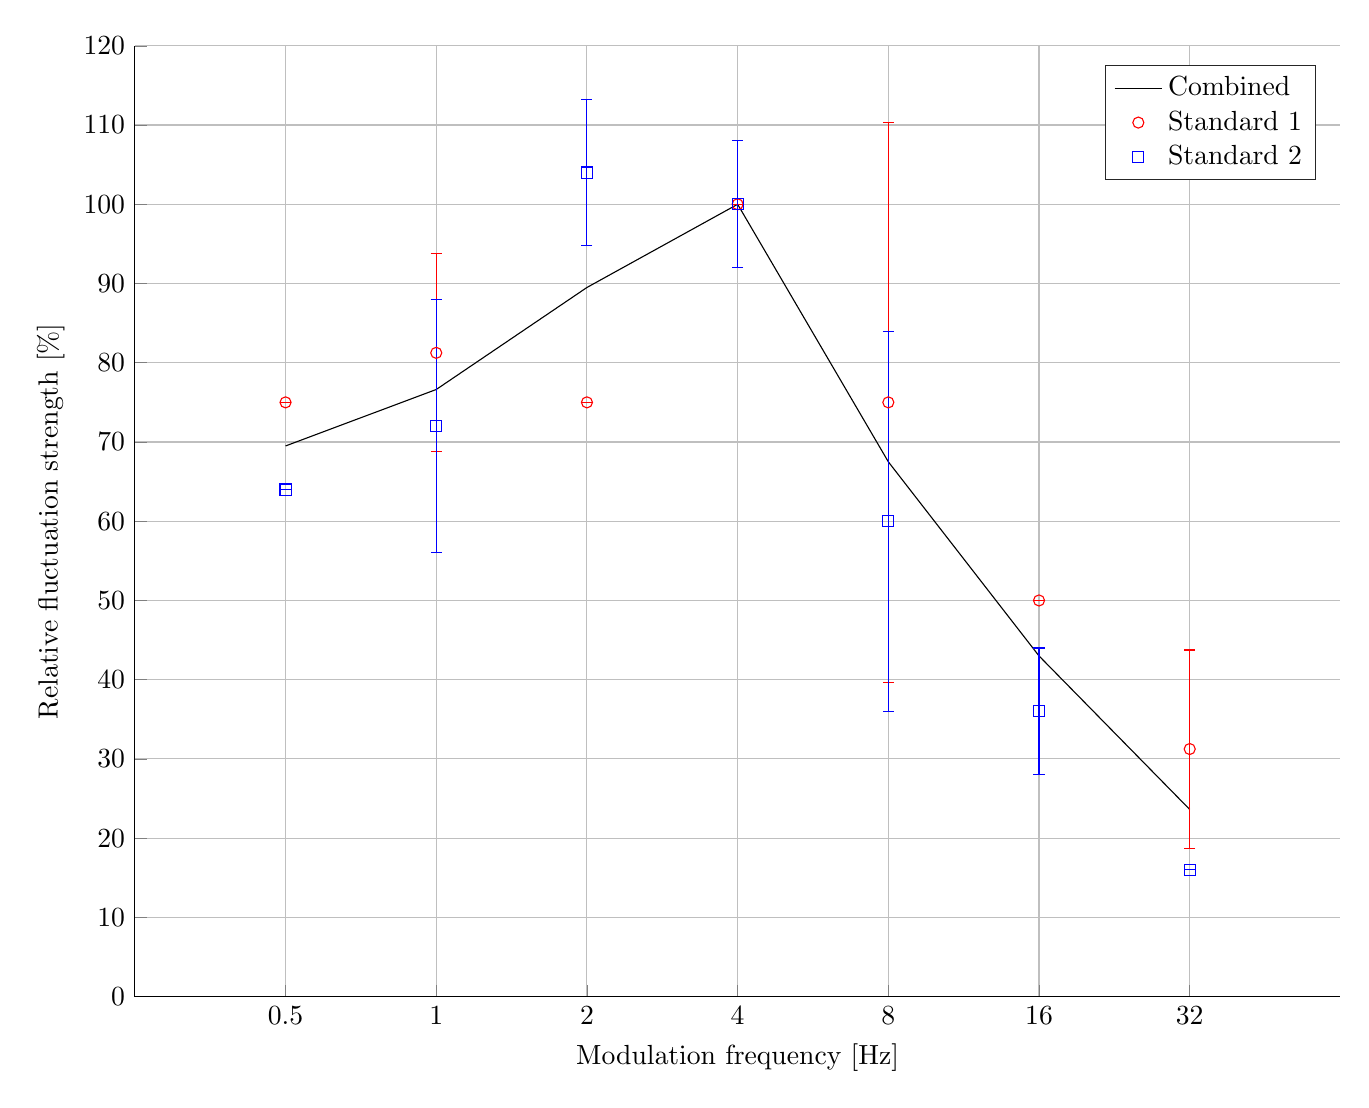
\begin{tikzpicture}

\begin{axis}[%
width=6.027778in,
height=4.754167in,
at={(1.011111in,0.641667in)},
scale only axis,
xmin=0,
xmax=8,
xtick={1,2,3,4,5,6,7},
xticklabels={{0.5},{1},{2},{4},{8},{16},{32}},
xlabel={Modulation frequency [Hz]},
xmajorgrids,
ymin=0,
ymax=120,
ylabel={Relative fluctuation strength [\%]},
ymajorgrids,
axis x line*=bottom,
axis y line*=left,
legend style={legend cell align=left,align=left,draw=white!15!black}
]
\addplot [color=black,solid]
  table[row sep=crcr]{%
1	69.5\\
2	76.625\\
3	89.5\\
4	100\\
5	67.5\\
6	43\\
7	23.625\\
};
\addlegendentry{Combined};

\addplot [color=red,only marks,mark=o,mark options={solid}]
 plot [error bars/.cd, y dir = both, y explicit]
 table[row sep=crcr, y error plus index=2, y error minus index=3]{%
1	75	0	0\\
2	81.25	12.5	12.5\\
3	75	0	0\\
4	100	0	0\\
5	75	35.3553390593274	35.3553390593274\\
6	50	0	0\\
7	31.25	12.5	12.5\\
};
\addlegendentry{Standard 1};

\addplot [color=blue,only marks,mark=square,mark options={solid}]
 plot [error bars/.cd, y dir = both, y explicit]
 table[row sep=crcr, y error plus index=2, y error minus index=3]{%
1	64	0	0\\
2	72	16	16\\
3	104	9.23760430703401	9.23760430703401\\
4	100	8	8\\
5	60	24	24\\
6	36	8	8\\
7	16	0	0\\
};
\addlegendentry{Standard 2};

\end{axis}
\end{tikzpicture}%
    }
    \caption{Relative fluctuation strength as a function of modulation
        frequency by standard used for FM tones with $f_c = 1.5$ kHz,
        $d_f = 700$ Hz, SPL $= 70$ dB (error bars indicate standard deviation)}
    \label{fig:fmstds}
\end{figure}

\begin{figure}[ht]
    \centering
    \resizebox{!}{10cm}{
        % This file was created by matlab2tikz.
% Minimal pgfplots version: 1.9
%
%The latest updates can be retrieved from
%  http://www.mathworks.com/matlabcentral/fileexchange/22022-matlab2tikz
%where you can also make suggestions and rate matlab2tikz.
%
\definecolor{mycolor1}{rgb}{0.00000,0.44700,0.74100}%
\definecolor{mycolor2}{rgb}{0.85000,0.32500,0.09800}%
%
\begin{tikzpicture}

\begin{axis}[%
width=6.027778in,
height=4.754167in,
at={(1.011111in,0.641667in)},
scale only axis,
xmin=0,
xmax=8,
xtick={1,2,3,4,5,6,7},
xticklabels={{0.5},{1},{2},{4},{8},{16},{32}},
xlabel={Modulation frequency [Hz]},
xmajorgrids,
ymin=0,
ymax=120,
ylabel={Relative fluctuation strength [\%]},
ymajorgrids,
axis x line*=bottom,
axis y line*=left,
legend style={legend cell align=left,align=left,draw=white!15!black}
]
\addplot [color=black,solid]
 plot [error bars/.cd, y dir = both, y explicit]
 table[row sep=crcr, y error plus index=2, y error minus index=3]{%
1	69.5	5.87974732207334	5.87974732207334\\
2	76.625	14.1818546036828	14.1818546036828\\
3	89.5	16.6390246966925	16.6390246966925\\
4	100	5.23722936566382	5.23722936566382\\
5	67.5	29.1008100034542	29.1008100034542\\
6	43	9.13392420751187	9.13392420751187\\
7	23.625	11.5503555913103	11.5503555913103\\
};
\addlegendentry{Experiment};

\addplot [color=mycolor1,solid]
  table[row sep=crcr]{%
1	21.5365239294711\\
2	42.4433249370277\\
3	58.3123425692695\\
4	100.125944584383\\
5	35.0125944584383\\
6	13.3501259445844\\
7	1.13350125944586\\
};
\addlegendentry{Fastl2007Psychoacoustics};

\addplot [color=mycolor2,solid]
  table[row sep=crcr]{%
1	12.6401850483713\\
2	29.1583754086958\\
3	50.4708417907444\\
4	80.12461467033\\
5	100\\
6	21.4971284748007\\
7	0.0494270541422769\\
};
\addlegendentry{Model};

\end{axis}
\end{tikzpicture}%
    }
    \caption{Comparison between relative fluctuation strength as a function of
        modulation frequency for FM tones using the experimental data,
        \citeauthor{Fastl2007Psychoacoustics} data and the proposed model
        (error bars indicate standard deviation)}
    \label{fig:fmcomp}
\end{figure}

\custombibliography

\end{document}
